\chapter{Конструкторский раздел}

В данном разделе будут приведены требования к входным, выходным параметрам и представлены схемы для классического алгоритма умножения матриц, алгоритма Винограда и его оптимизированной версии.

В качестве оптимизирующих операций были выполнены:

\begin{itemize}[label=--]
    \item замена умножения на 2 на двоичный сдвиг;
    \item использование инкремента <<+=>>;
    \item вынос начальной итерации из каждого внешнего цикла;
\end{itemize}

\section{Требования к входным и выходным параметрам}

Требования к входным и выходным параметрам:
\begin{itemize}[label=--]
    \item в качестве входных параметров алгоритм принимает две матрицы;
    \item корректными входными параметрами являются совместимые матрицы, в каждой из которых есть по крайней мере 1 строка и 1 столбец;
    \item выходным параметром является матрица, полученная в результате умножения первой матрицы на вторую.
\end{itemize}

\section{Схемы алгоритмов}

На рисунках~\ref{fig:classic_mult_scheme}~и~\ref{fig:winograd_opt_scheme_2} представлены схемы различных алгоритмов умножения матриц.

\begin{figure}[H]
\centering
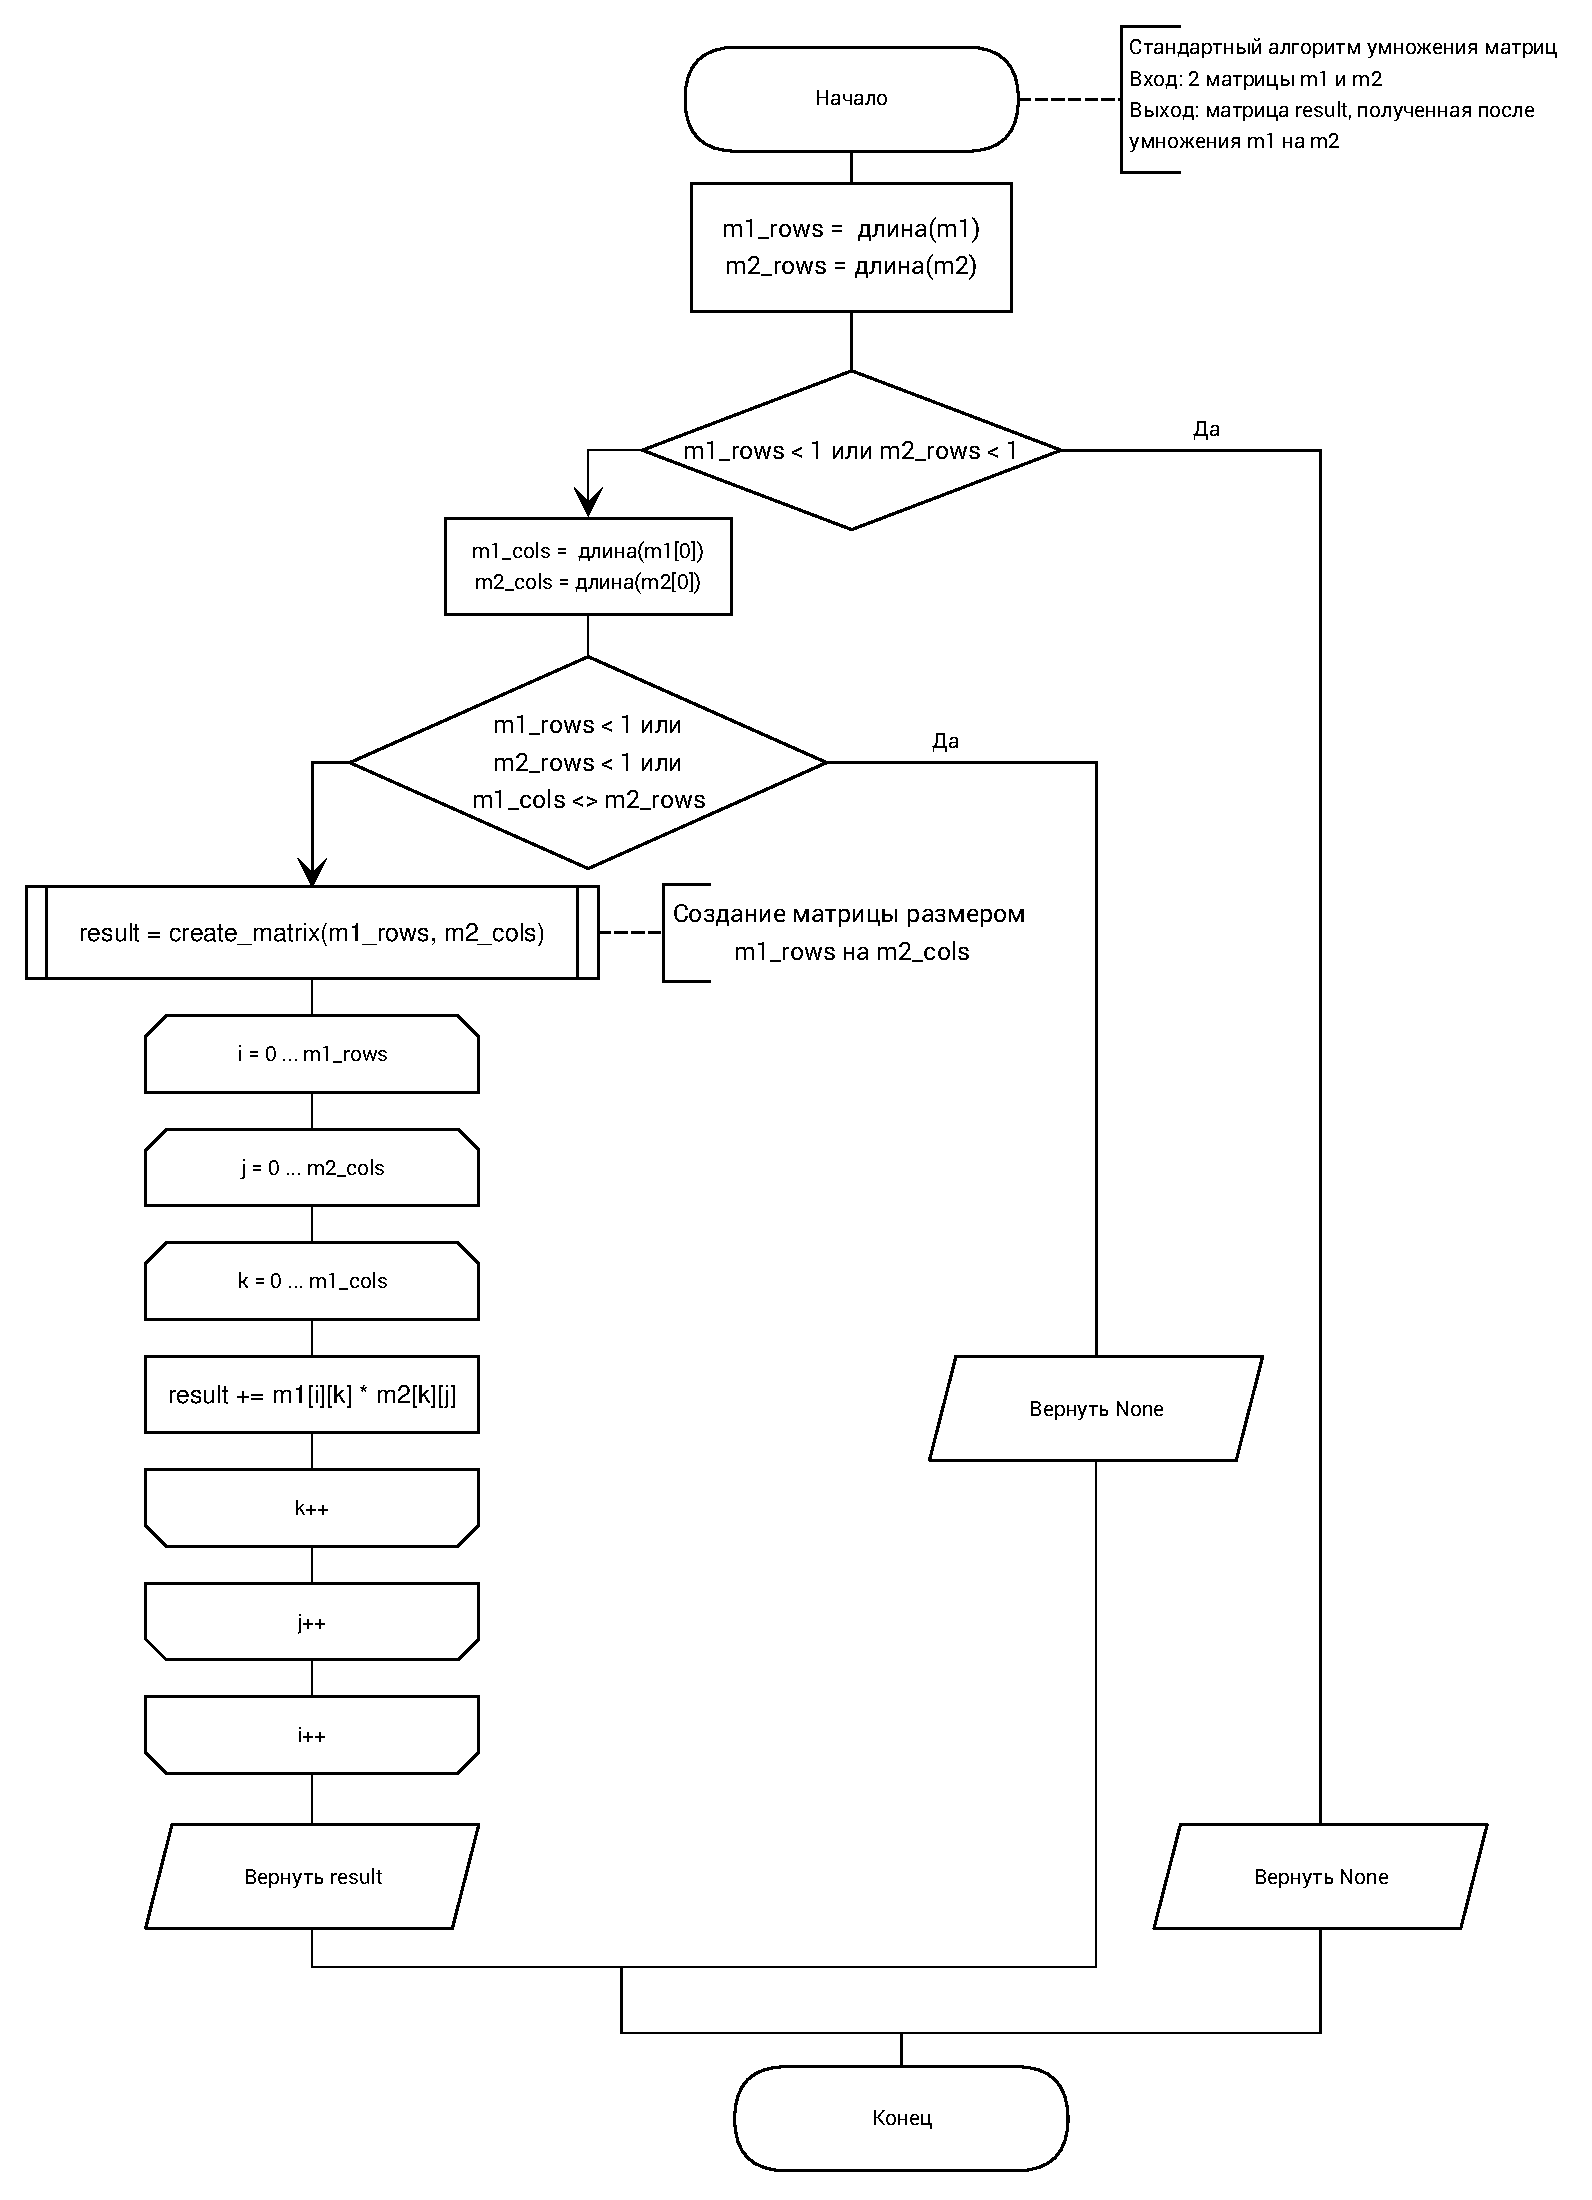
\includegraphics[width=\textwidth]{inc/img/standard_mult.pdf}
\caption{Схема классического алгоритма умножения матриц}
\label{fig:classic_mult_scheme}
\end{figure}

\begin{figure}[H]
\centering
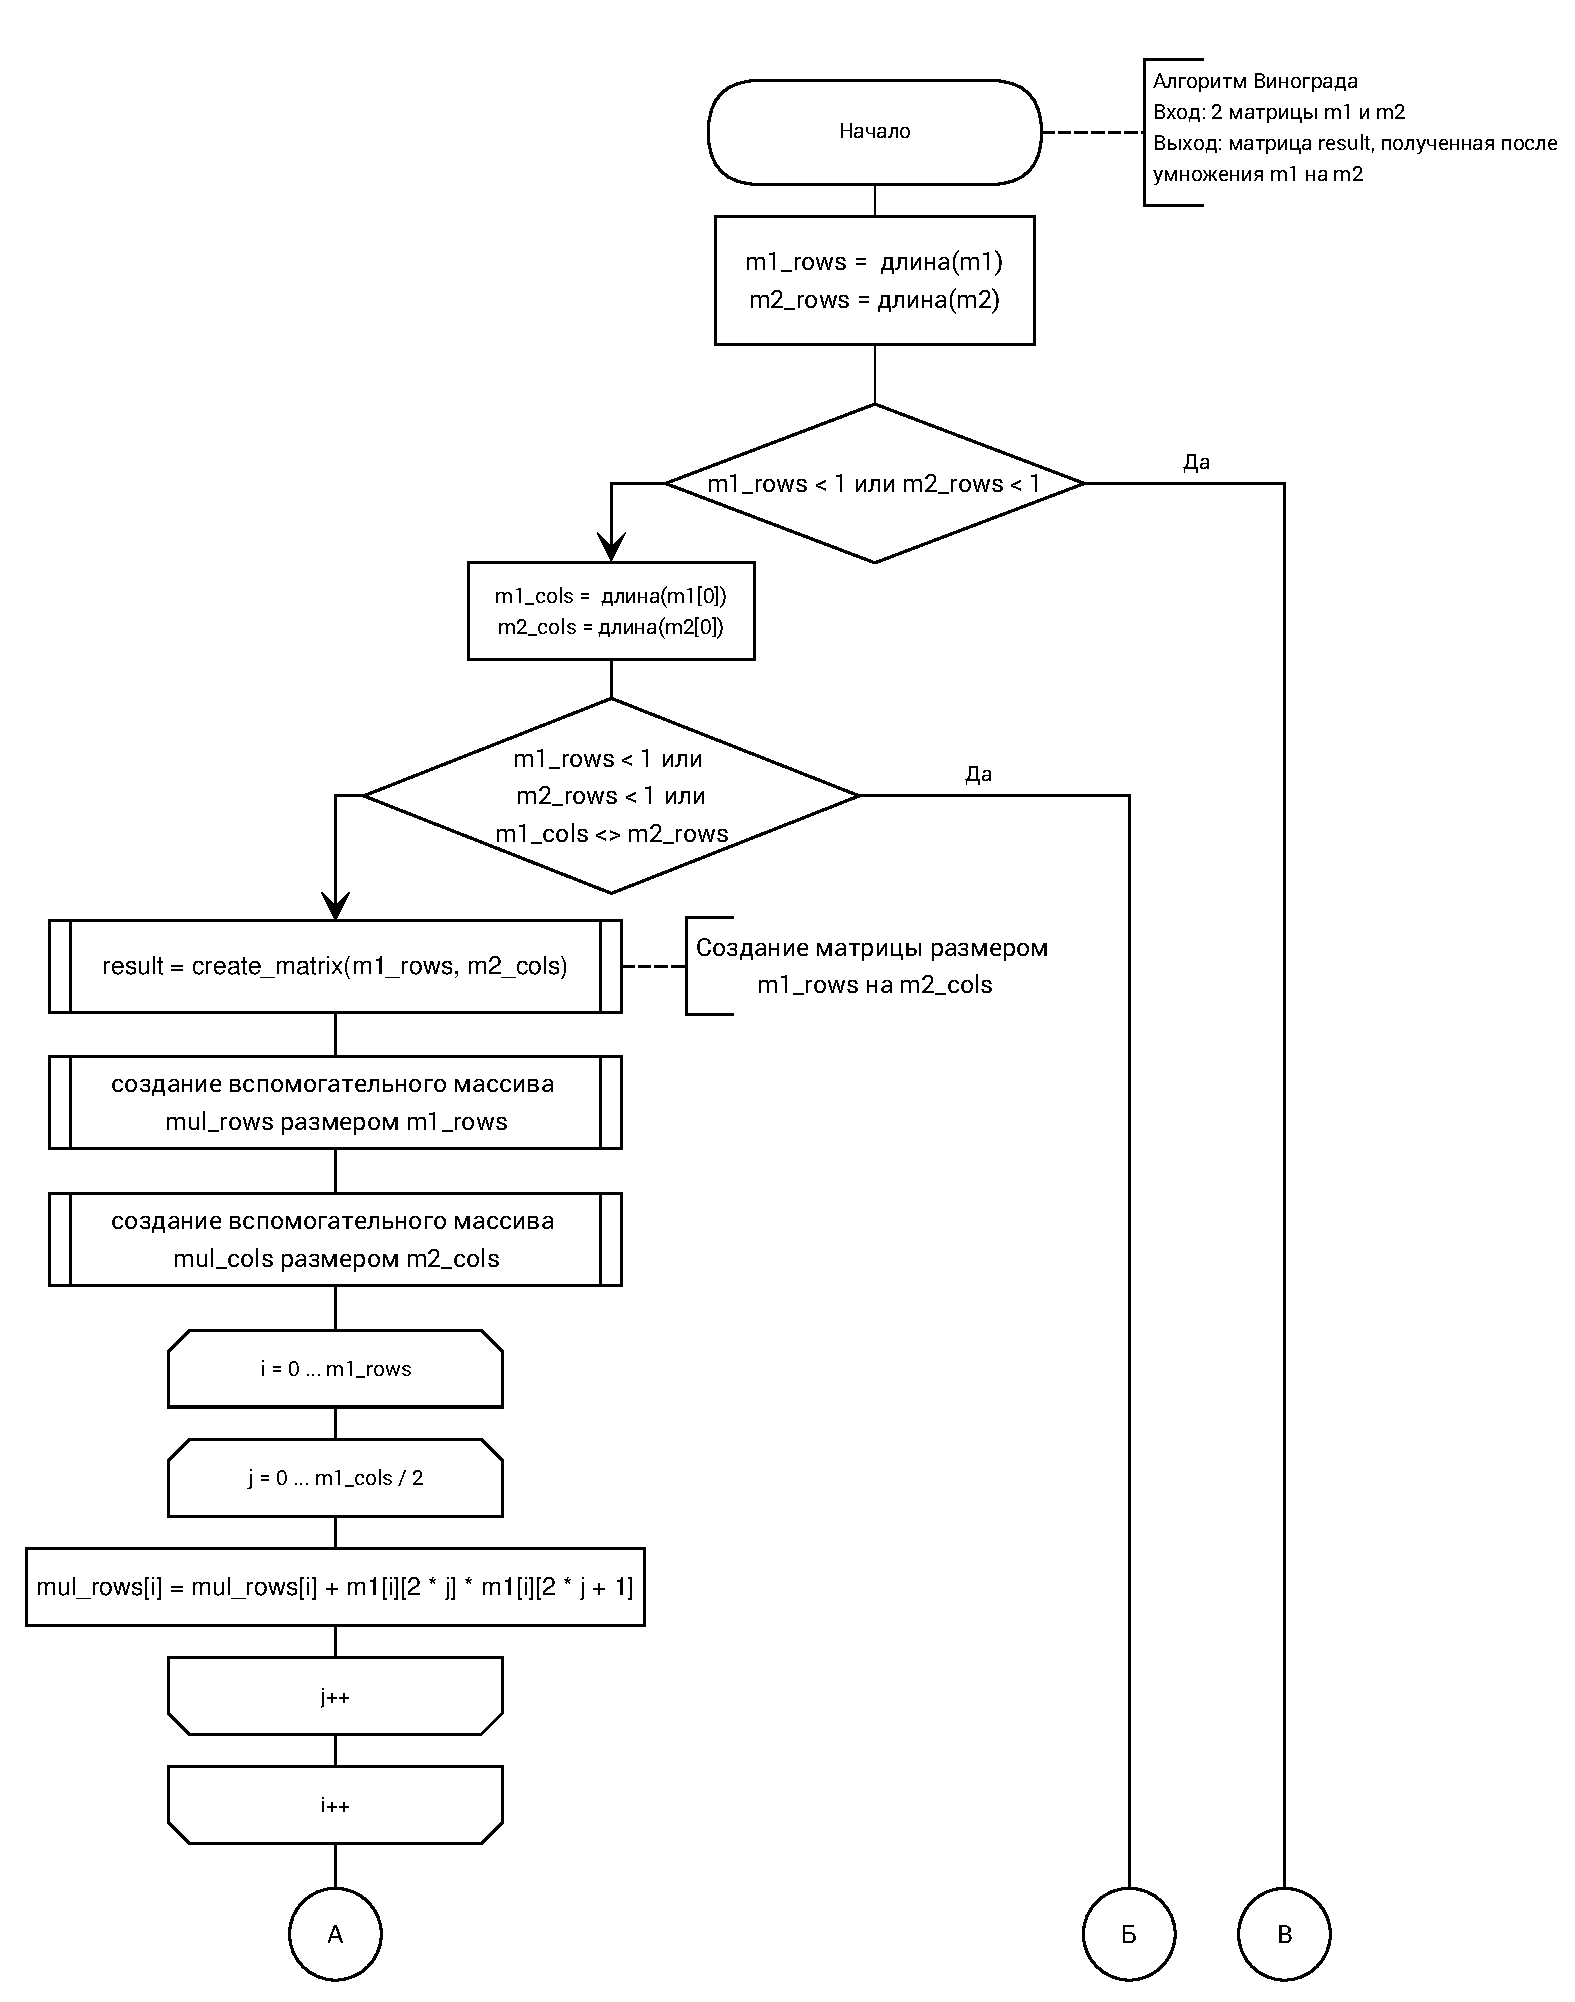
\includegraphics[width=\textwidth]{inc/img/winograd_1.pdf}
\caption{Схема алгоритма Винограда. Часть 1}
\label{fig:winograd_scheme_1}
\end{figure}

\begin{figure}[H]
\centering
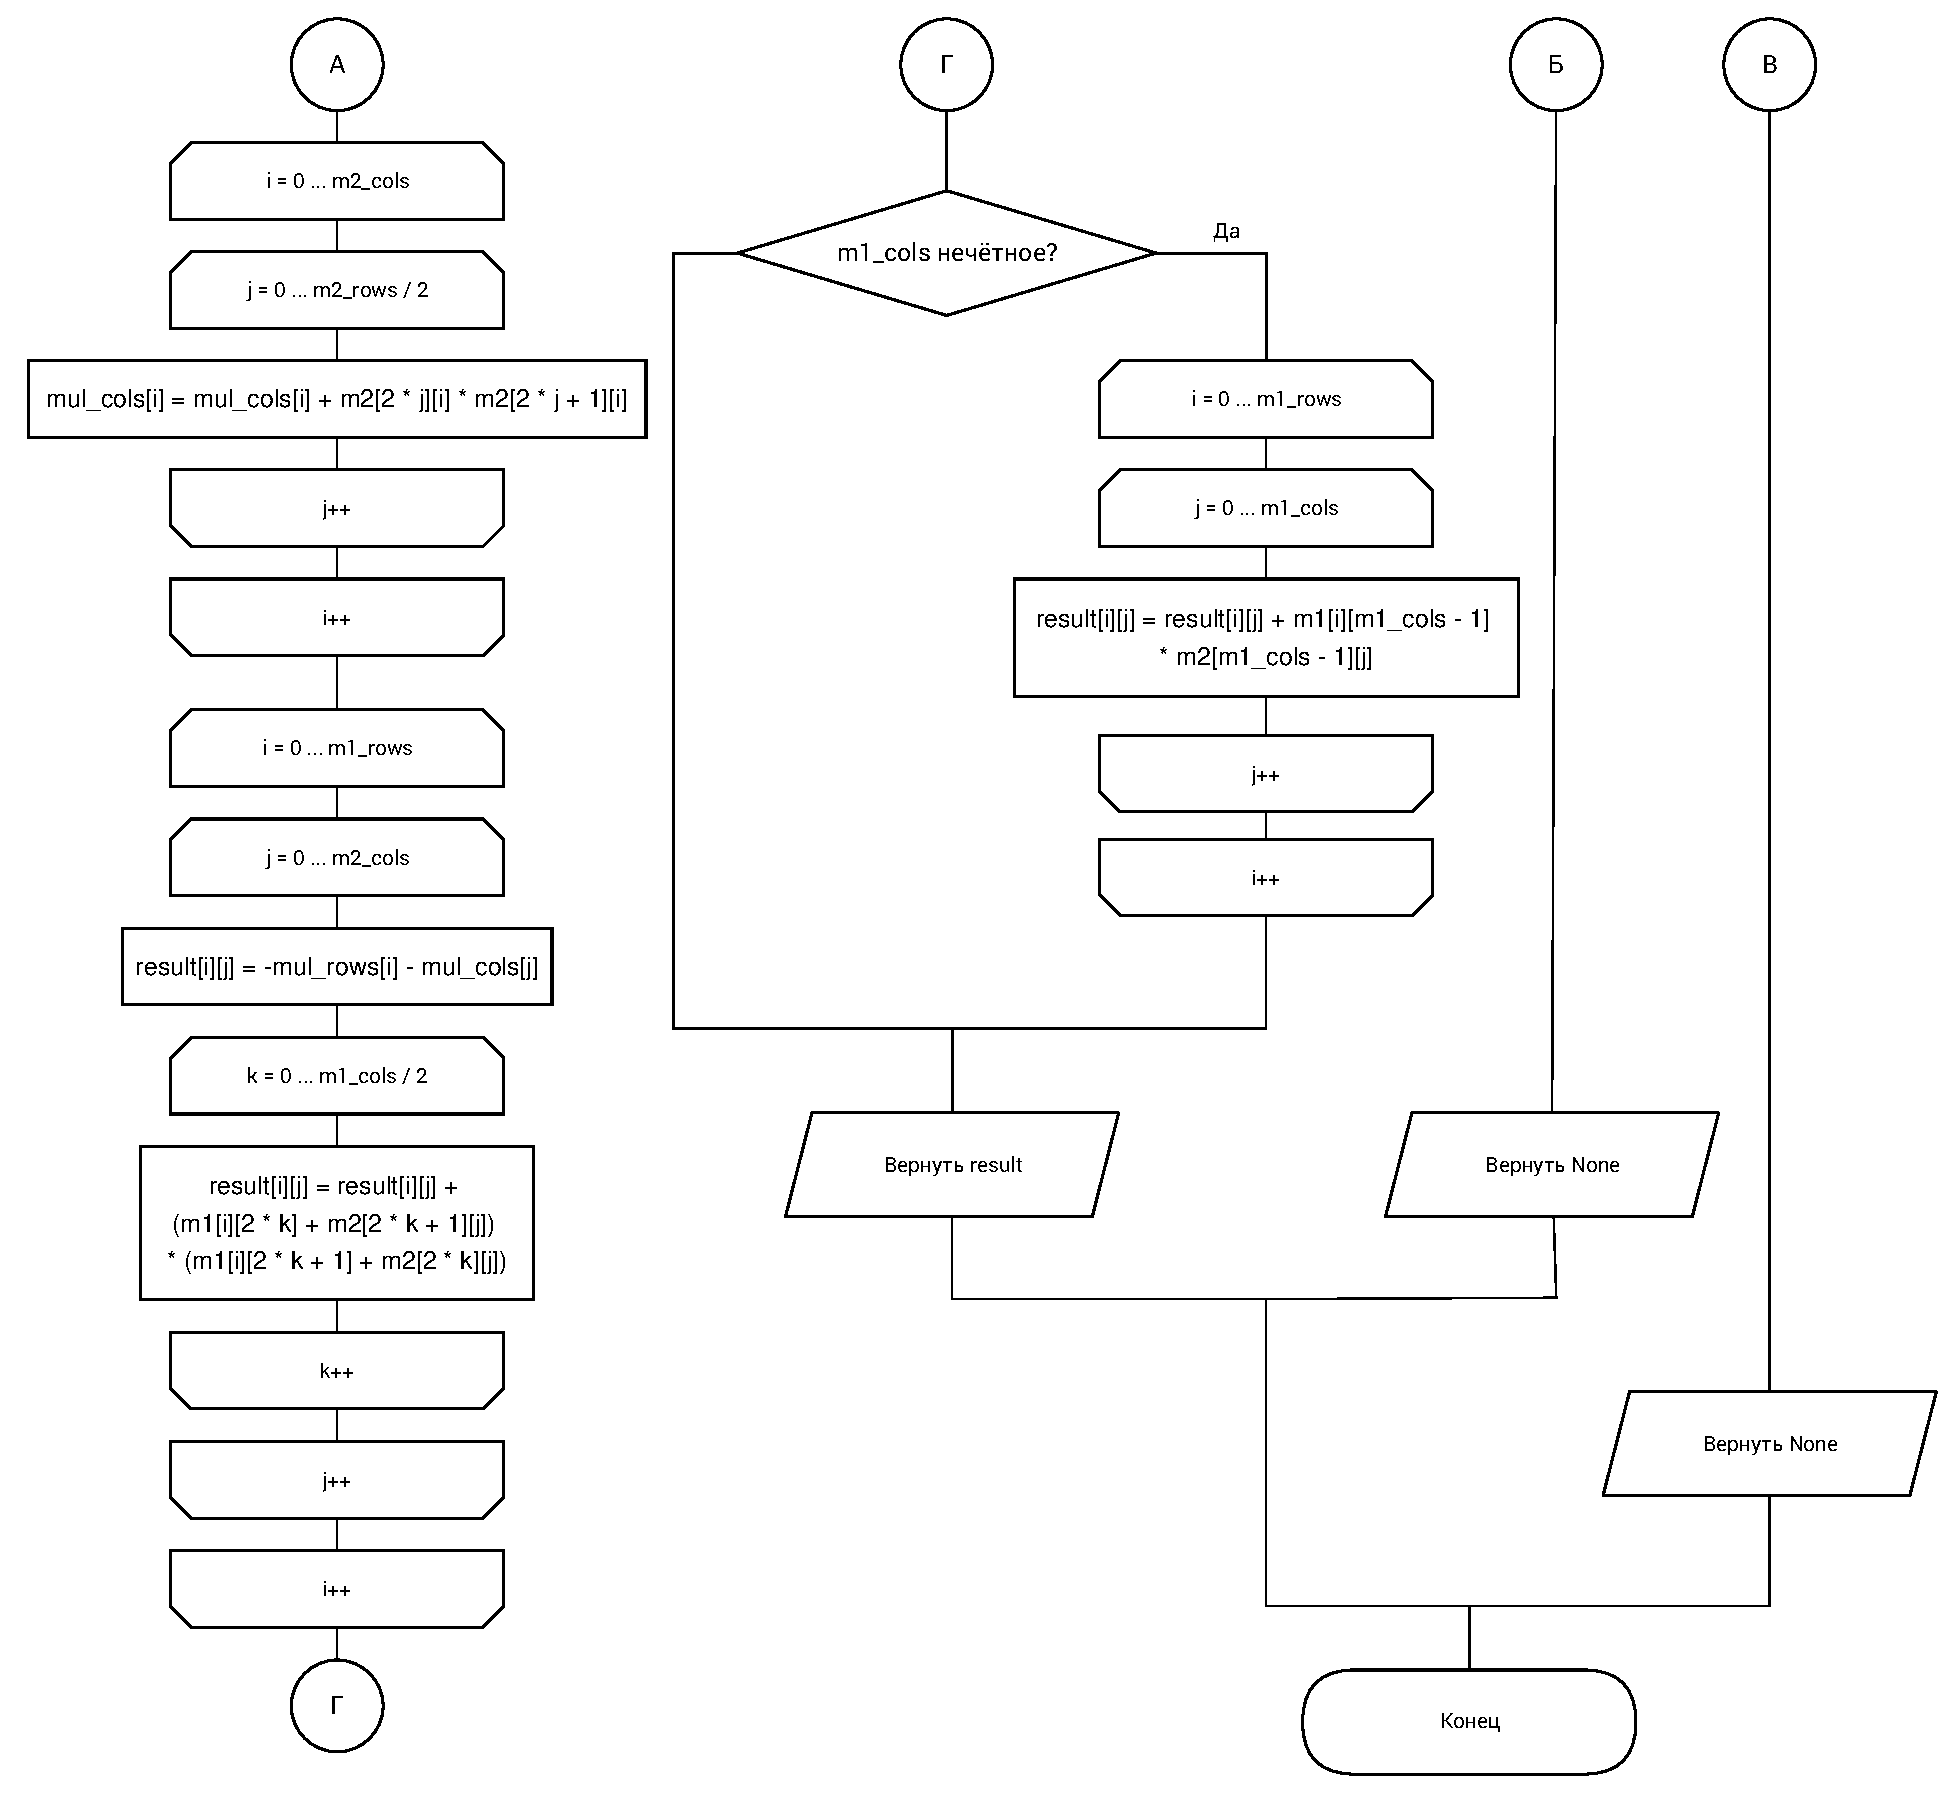
\includegraphics[width=\textwidth]{inc/img/winograd_2.pdf}
\caption{Схема алгоритма Винограда. Часть 2}
\label{fig:winograd_scheme_2}
\end{figure}

\begin{figure}[H]
\centering
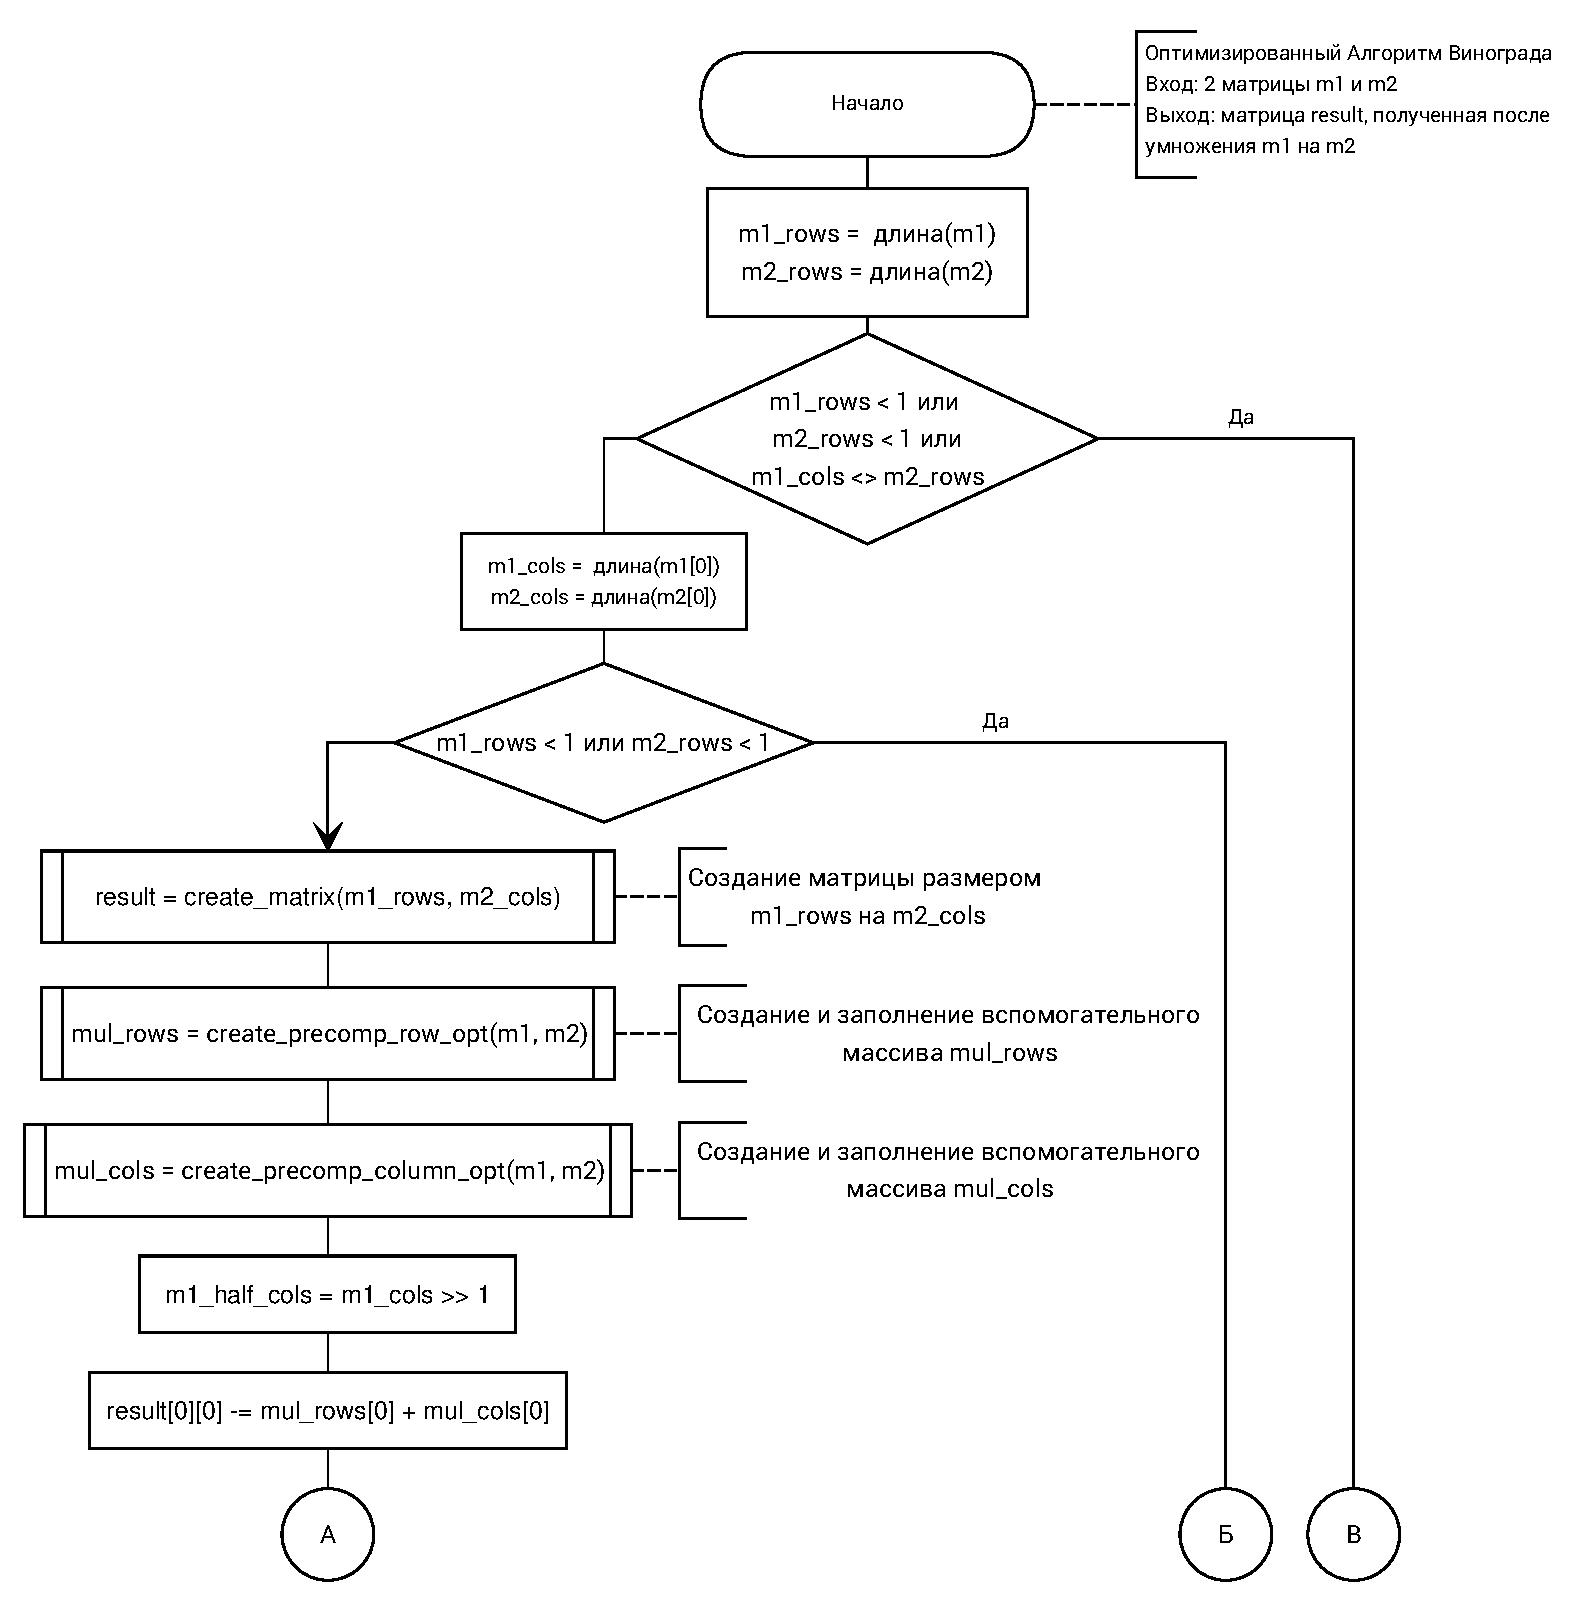
\includegraphics[width=\textwidth]{inc/img/winograd_opt_1.pdf}
\caption{Схема оптимизированного алгоритма Винограда. Часть 1}
\label{fig:winograd_opt_scheme_1}
\end{figure}

\begin{figure}[H]
\centering
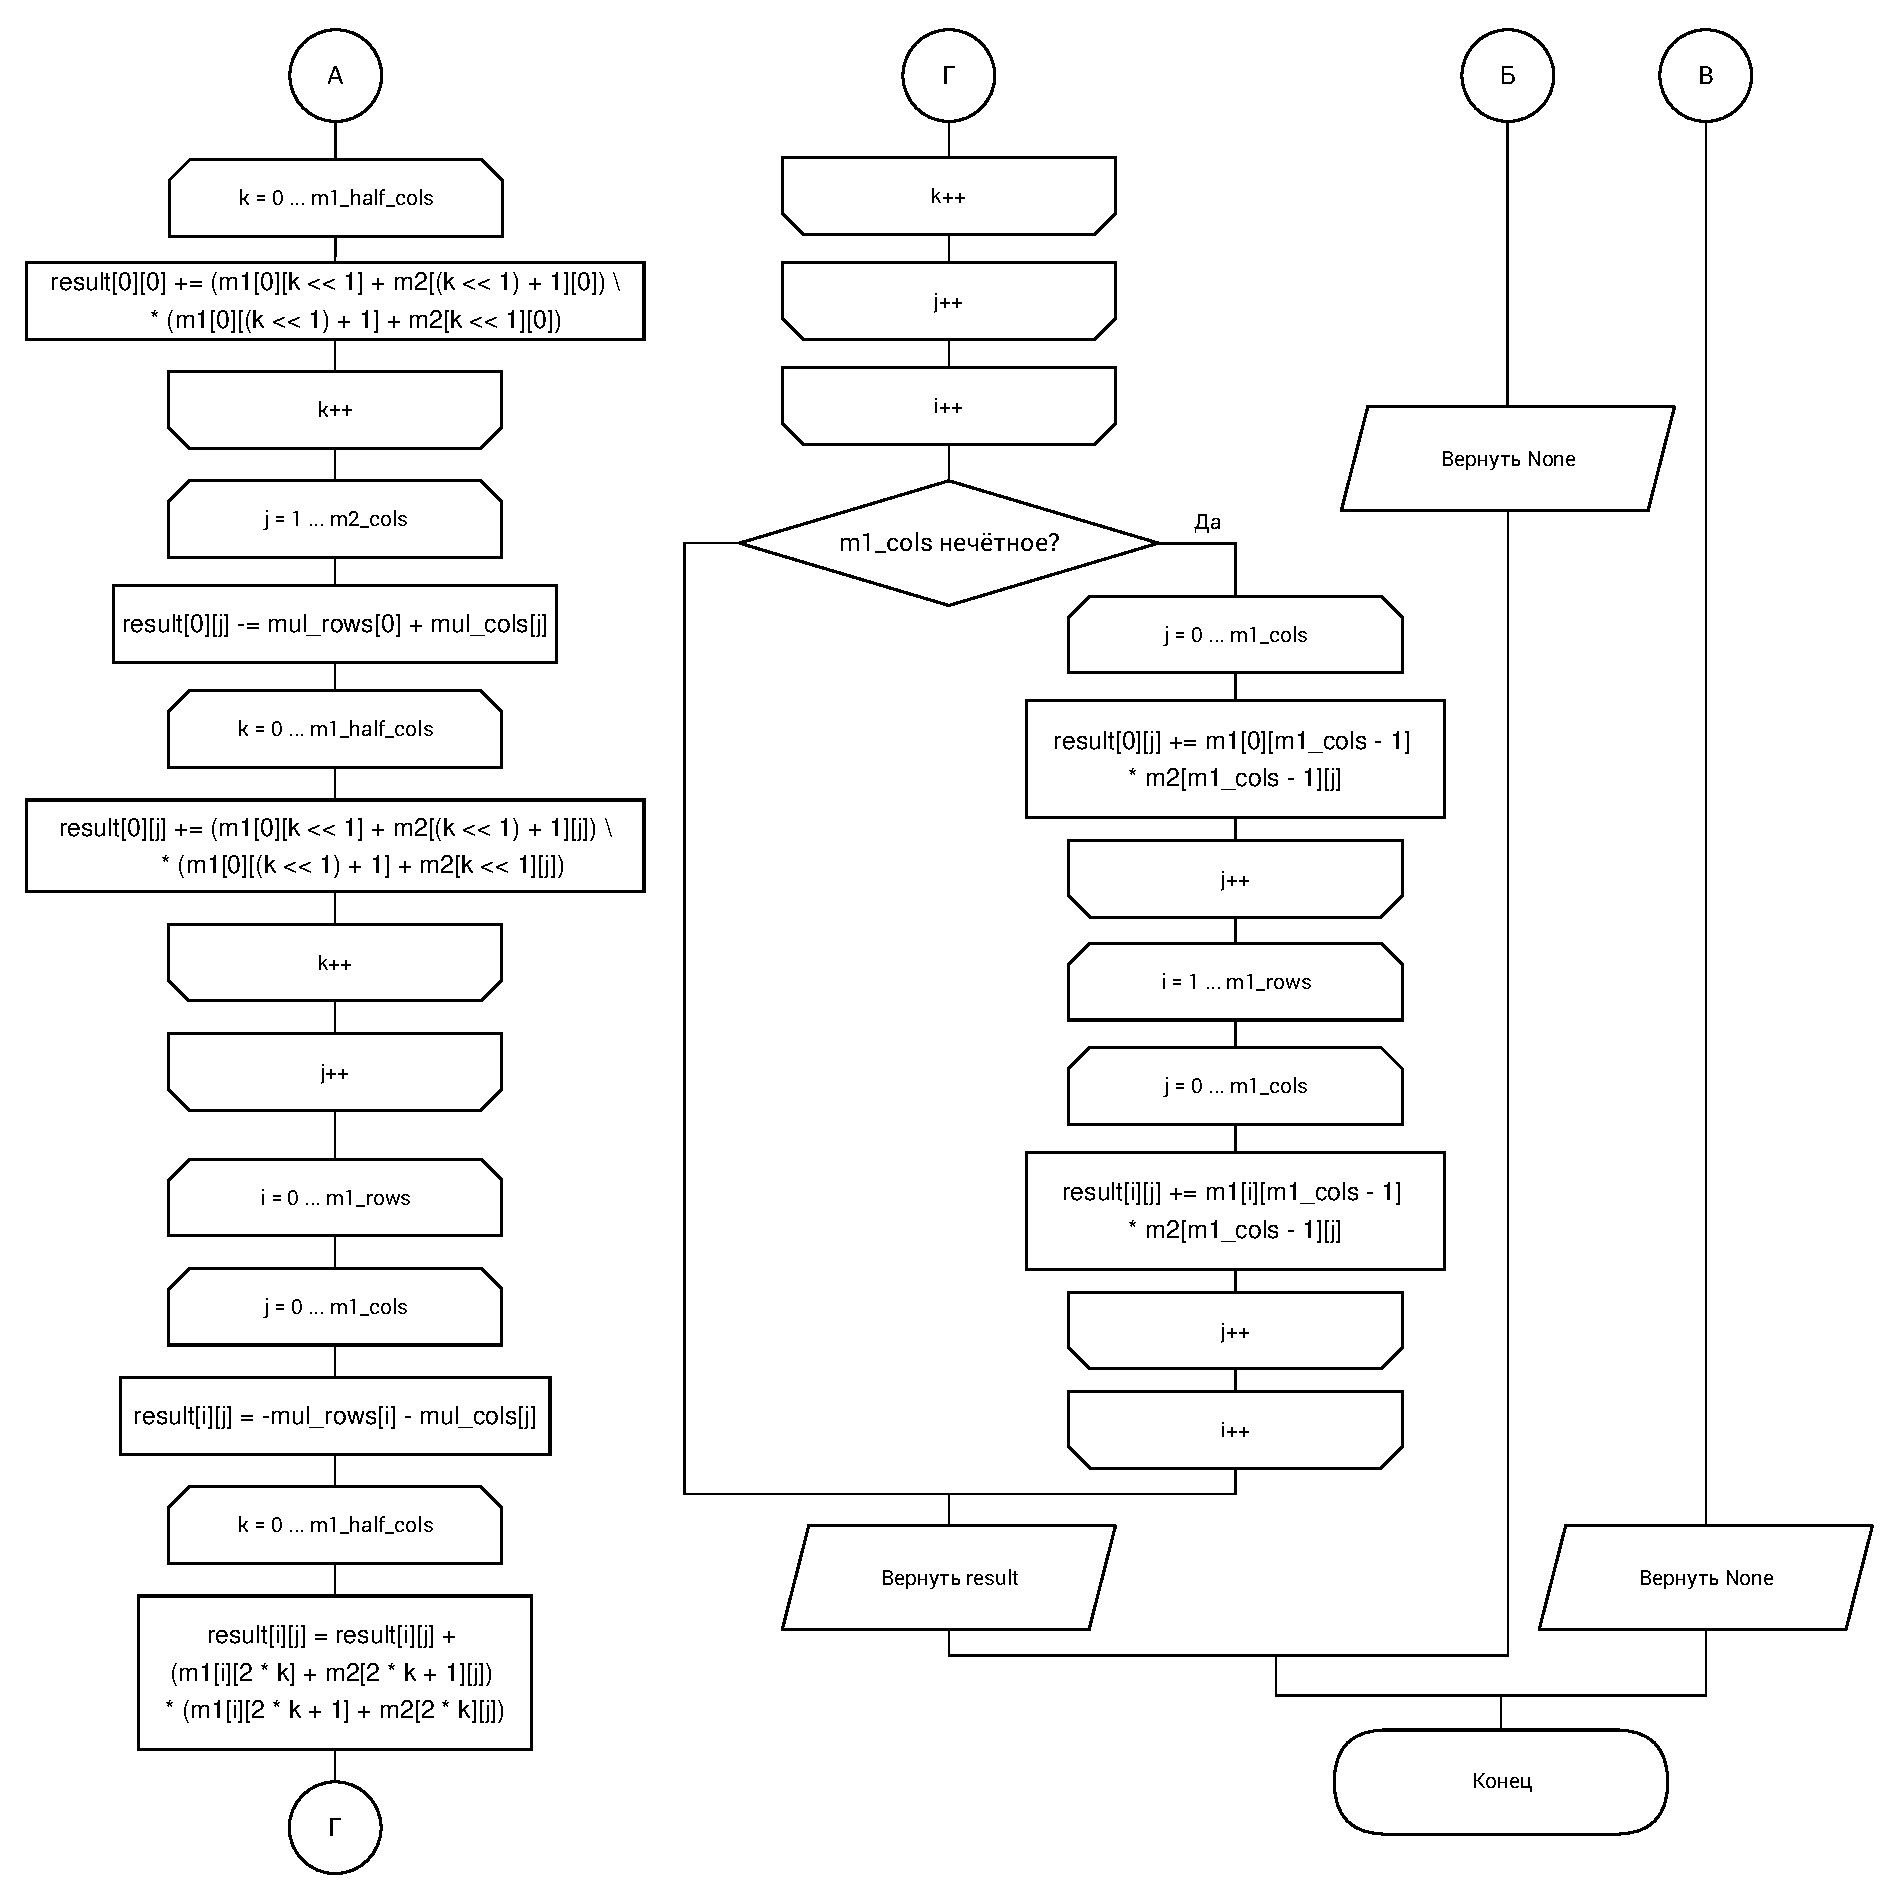
\includegraphics[width=\textwidth]{inc/img/winograd_opt_2.pdf}
\caption{Схема оптимизированного алгоритма Винограда. Часть 2}
\label{fig:winograd_opt_scheme_2}
\end{figure}

На рисунке~\ref{fig:winograd_opt_scheme_3} представлены схемы алгоритмов заполнения вспомогательных массивов попарными операциями умножения.

\begin{figure}[H]
\centering
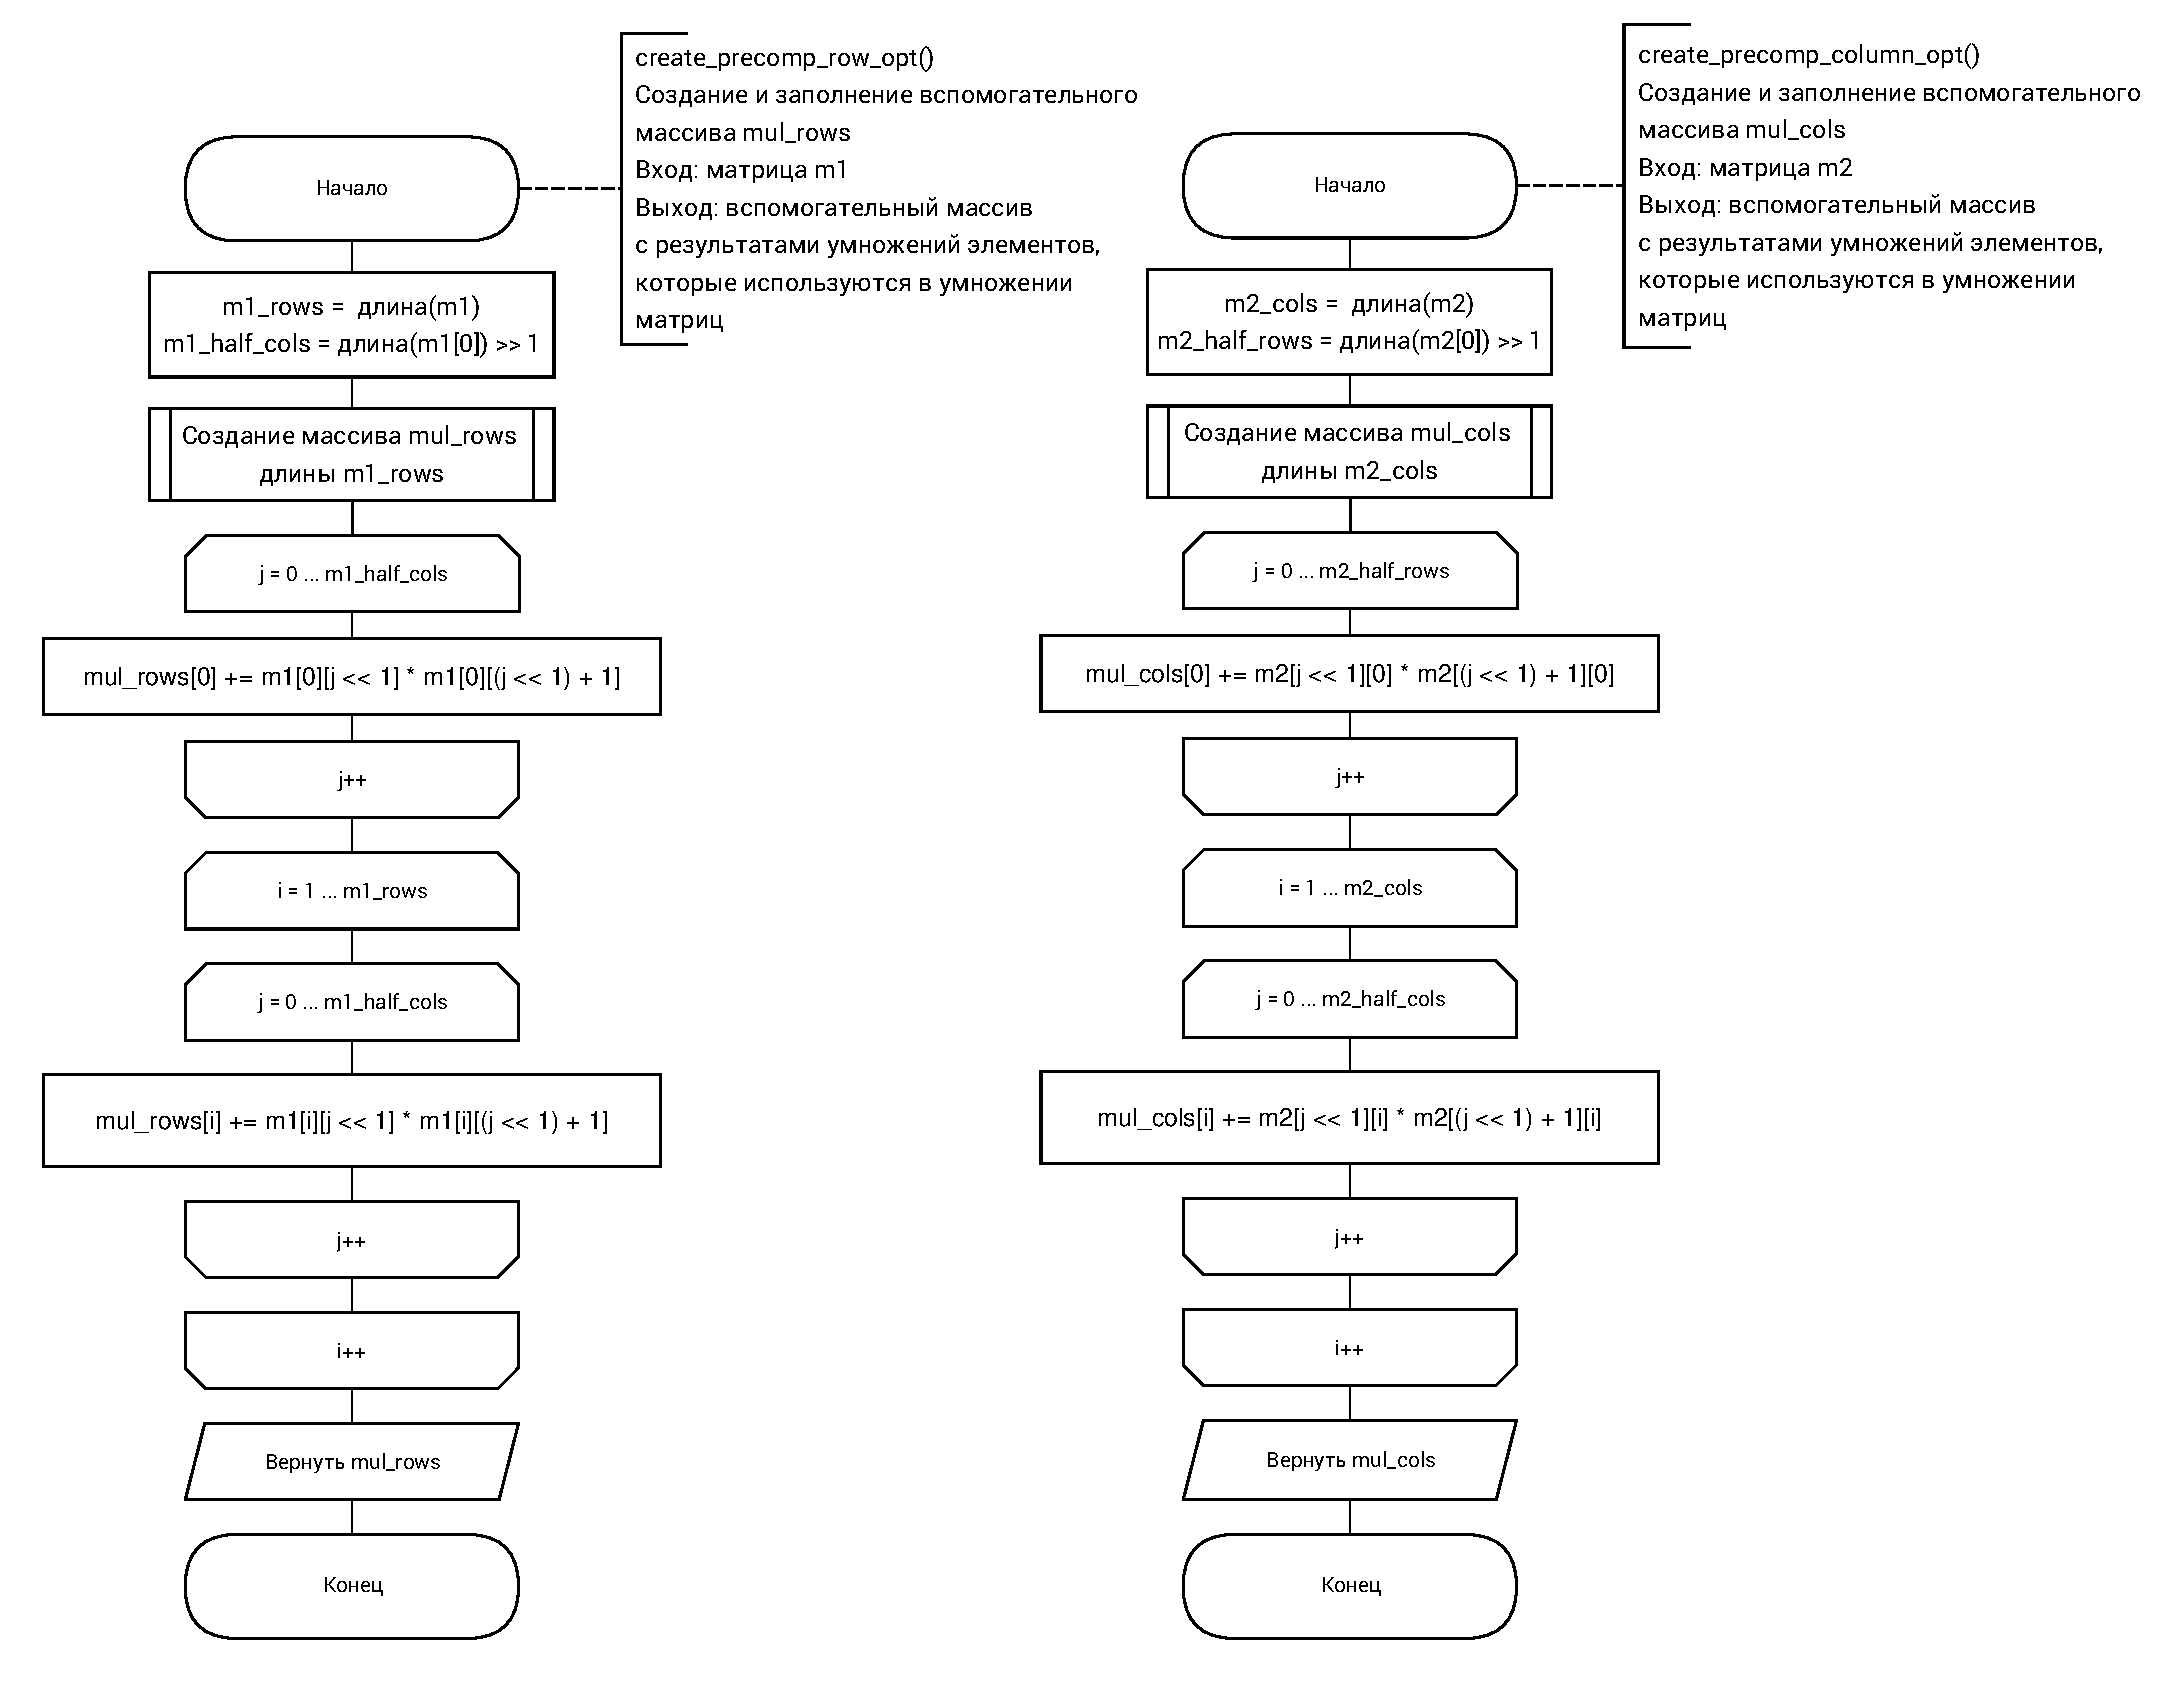
\includegraphics[width=\textwidth]{inc/img/winograd_opt_3.pdf}
\caption{Схемы алгоритмов заполнения вспомогательных массивов}
\label{fig:winograd_opt_scheme_3}
\end{figure}

\section{Оценка трудоёмкости}

\subsection{Модель вычислений}\label{sub:model}

Операции, имеющие единичную стоимость:
\begin{equation}
    \begin{gathered}
        +, -, =, +=, -=, ==, !=, <, >, <=, >=, [idx], ++, {-}-,\\
        \&\&, >>, <<, ||, \&, |
    \end{gathered}
\end{equation}

Операции, имеющие двойную стоимость:
\begin{equation}
    *, /, \%, *=, /=, \%=, len()
\end{equation}

Трудоёмкость условного оператора:
\begin{equation}
    f_{if} = f_{\text{условия}} + 
    \begin{cases}
        \text{min}(f_1, f_2), & \text{лучший случай}\\
        \text{max}(f_1, f_2), & \text{худший случай}
    \end{cases}
\end{equation}

Трудоёмкость цикла:
\begin{equation}
    \begin{gathered}
        f_{loop} = f_{\text{инициализация}} + f_{\text{сравнения}} + N \times (f_{\text{тело}} +\\
        + f_{\text{инкремент}} + f_{\text{сравнения}})
    \end{gathered}
\end{equation}

Трудоёмкость вызова функции равна нулю.

\subsection{Трудоёмкость стандартного алгоритма}

Стоимость начальной проверки значений и инициализации переменных:

\begin{equation}
    \label{eq:std_init}
    f_{init} = 3 \cdot 2 + 3 + (2 + 1 + 1) \cdot 2 + 5 + (2 + m \cdot (2 + p)). 
\end{equation}

Стоимость основного цикла рассчитывается по формуле~(\ref{eq:std_main_loop}).

\begin{equation}
    \label{eq:std_main_loop}
    f_{loop} = 2 + m \cdot(4 + p \cdot (4 + n \cdot (2 + 9)))
\end{equation}

Итоговая трудоёмкость рассчитывается по формуле~(\ref{eq:std_full}).

\begin{equation}
    \label{eq:std_full}
    \begin{gathered}
        f = f_{init} + f_{loop} = 26 + 6\cdot m + 5 \cdot m \cdot p \\
        + 11 \cdot m \cdot n \cdot p \approx 11 \cdot m \cdot n \cdot p = O(N^3)
    \end{gathered}
\end{equation}

\subsection{Трудоёмкость алгоритма Винограда}

Стоимость начальной проверки значений и инициализации переменных совпадает со стоимостью одноимённого пункта в стандартном алгоритме:

\begin{equation}
    \label{eq:winograd_init}
    \begin{gathered}
        f_{init} = 3 \cdot 2 + 3 + (2 + 1 + 1) \cdot 2 + 5 + (2 + m \cdot (2 + p)) \\
        = 24 + 2 \cdot m + m \cdot p.
    \end{gathered} 
\end{equation}

Стоимости инициализации вспомогательных массивов вычисляются по формулам~(\ref{eq:row_init})~и~(\ref{eq:col_init}.

\begin{equation}
    \label{eq:row_init}
    f_{row\_init} = 2 + 2 \cdot m + 2 + m \cdot (4 + 2 + \frac{n}{2} \cdot (1 + 1 + 15)).
\end{equation}

\begin{equation}
    \label{eq:col_init}
    f_{col\_init} = 2 + 2 \cdot p + 2 + p \cdot (4 + 2 + \frac{n}{2} \cdot (1 + 1 + 15)).
\end{equation}

Стоимость основного цикла в алгоритме Винограда вычисляется по формуле~(\ref{eq:winograd_loop}).

\begin{equation}
    \label{eq:winograd_loop}
    \begin{gathered}
        f_{loop} = 2 + m \cdot (2 + 2 + p \cdot (13 + \frac{n}{2} \cdot 30)) \\
        = 2 + 4 \cdot m + 13 \cdot m \cdot p + 15 \cdot m \cdot n \cdot p
    \end{gathered}
\end{equation}

Стоимость учёта нечётности в алгоритме Винограда рассчитывается по формуле~(\ref{eq:winograd_check}).

\begin{equation}
    \label{eq:winograd_check}
    \begin{gathered}
        f_{check} = 3 + \begin{cases}
            0, & \text{чётная} \\
            2 + 4 \cdot m + 16 \cdot m \cdot p, & \text{нечётная}
        \end{cases}
    \end{gathered}
\end{equation}

Итоговая трудоёмкость алгоритма Винограда вычисляется по формуле~(\ref{eq:winograd_main}).

\begin{equation}
    \label{eq:winograd_main}
    f = f_{init} + f_{row\_init} + f_{col\_init} + f_{loop} + f_{check}
\end{equation}

В лучшем случае трудоёмкость алгоритма составляет:

\begin{equation}
    \begin{gathered}
        f = 37 + 14 \cdot m +  8 \cdot p + 14 \cdot m \cdot p 
        + 8.5 \cdot m \cdot n + 8.5 \cdot n \cdot p \\
        + 15 \cdot m \cdot n \cdot p \approx 15 \cdot m \cdot n \cdot p = O(N^3)
    \end{gathered}
\end{equation}

В худшем случае трудоёмкость алгоритма составляет:

\begin{equation}
    \begin{gathered}
        f = 39 + 18 \cdot m +  8 \cdot p + 30 \cdot m \cdot p 
        + 8.5 \cdot m \cdot n + 8.5 \cdot n \cdot p \\
        + 15 \cdot m \cdot n \cdot p \approx 15 \cdot m \cdot n \cdot p = O(N^3)
    \end{gathered}
\end{equation}

\subsection{Трудоёмкость оптимизированного алгоритма Винограда}

Стоимость начальной проверки значений и инициализации переменных вычисляется по формуле:

\begin{equation}
    \begin{gathered}
        f_{init} = 2 + 3 \cdot 2 + 3 + (2 + 1 + 1) \cdot 2 + 5 + (2 + m \cdot (2 + p)) \\
        = 26 + 2 \cdot m + m \cdot p.
    \end{gathered} 
\end{equation}

Стоимости инициализации вспомогательных массивов вычисляются по формулам~(\ref{eq:row_init_opt})~и~(\ref{eq:col_init_opt}.

\begin{equation}
    \label{eq:row_init_opt}
    \begin{gathered}
        f_{row\_init} = 13 + 2 \cdot m + \frac{n}{2} \cdot 13 + (m-1)\cdot(4 + \frac{n}{2}\cdot 13) \\ = 9 + 6 \cdot m + 6.5 \cdot m \cdot n
    \end{gathered} 
\end{equation}

\begin{equation}
    \label{eq:col_init_opt}
    \begin{gathered}
        f_{col\_init} = 13 + 2 \cdot p + \frac{n}{2} \cdot 13 + (p-1)\cdot(4 + \frac{n}{2}\cdot 13) \\ = 9 + 6 \cdot p + 6.5 \cdot p \cdot n
    \end{gathered} 
\end{equation}

Стоимость основного цикла оптимизированного алгоритма Винограда с учётом выноса первых итераций каждого внешнего цикла вычисляется по формуле:

\begin{equation}
    \begin{gathered}
        f_{main} = 6 + 2 + \frac{n}{2} \cdot 23 + 2 + (p - 1)\cdot(10 + \frac{n}{2}\cdot 23)
        + 2 \\ + (m - 1) \cdot (4 + p \cdot (10 + \frac{n}{2} \cdot 23)) = -2 + 4\cdot m + 10 \cdot m \cdot p + 11.5 \cdot m \cdot n \cdot p
    \end{gathered}
\end{equation}

Стоимость учёта нечётности в алгоритме Винограда рассчитывается по формуле~(\ref{eq:winograd_opt_check}).

\begin{equation}
    \label{eq:winograd_opt_check}
    \begin{gathered}
        f_{check} = 3 + \begin{cases}
            0, & \text{чётная} \\
            4 + 13 \cdot p + (m - 1)(4 + 13 \cdot p), & \text{нечётная}
        \end{cases}
    \end{gathered}
\end{equation}

Итоговая трудоёмкость оптимизированного алгоритма Винограда вычисляется по формуле~(\ref{eq:winograd_main}).

\begin{equation}
    \label{eq:winograd_main}
    f = f_{init} + f_{row\_init} + f_{col\_init} + f_{main} + f_{check}
\end{equation}

В лучшем случае трудоёмкость алгоритма составляет:

\begin{equation}
    \begin{gathered}
        f = 45 + 12\cdot m + 6 \cdot p + 11\cdot m\cdot p + 6.5 \cdot m \cdot n \\ + 6.5 \cdot n \cdot p + 11.5 \cdot m \cdot n \cdot p \approx 11.5 \cdot m \cdot n \cdot p = O(N^3)
    \end{gathered}
\end{equation}

В худшем случае трудоёмкость алгоритма составляет:

\begin{equation}
    \begin{gathered}
        f = 45 + 16\cdot m + 6 \cdot p + 24\cdot m\cdot p + 6.5 \cdot m \cdot n \\ + 6.5 \cdot n \cdot p + 11.5 \cdot m \cdot n \cdot p \approx 11.5 \cdot m \cdot n \cdot p = O(N^3)
    \end{gathered}
\end{equation}

\section*{Вывод}

В данном разделе были приведены схемы алгоритмов умножения матриц и рассчитана их трудоёмкость. В рамках модели вычислений, определённой в подразделе~\ref{sub:model}, все приведённые алгоритмы имеют кубическую сложность. Оптимизация уменьшила коэффициент при старшем члене в формуле трудоёмкости для алгоритма Винограда до $11.5$, но наименьший коэффициент при старшем члене все же принадлежит стандартному алгоритму ($11$).